% INTEGRATED_REVISION_V2
\documentclass[11pt,a4paper]{article}
\usepackage[margin=25mm]{geometry}
\usepackage[T1]{fontenc}
\usepackage{mathpazo,amsmath,amssymb,graphicx,booktabs,longtable,array,caption,setspace,microtype}
\usepackage[hidelinks]{hyperref}
\usepackage{fancyhdr}
\usepackage{placeins}
\usepackage[mathlines]{lineno}
\setstretch{1.15}
\setlength{\parskip}{4pt}
\setlength{\parindent}{0pt}
\captionsetup{font=small,labelfont=bf}
\pagestyle{fancy}\fancyhf{}\fancyhead[L]{\small GBD 2023: infertility contrasts}\fancyhead[R]{\small Additional file 1}\fancyfoot[C]{\thepage}
\setlength{\headheight}{14pt}
\setlength{\emergencystretch}{2em}
\newcommand{\ASPR}{\mathrm{ASPR}}
\title{Additional file 1: Reference-country composition and PCOS-attributed infertility}
\author{Companion to the revised comparator manuscript}
\date{29 October 2026}

\begin{document}\maketitle
\renewcommand{\thetable}{S\arabic{table}}\setcounter{table}{0}
\renewcommand{\thefigure}{S\arabic{figure}}\setcounter{figure}{0}
\section{Scope and computational audit}
This supplement accompanies the focused 29 October 2026 revision. Every numerical table and figure below is regenerated by \texttt{code/revision\_analysis.py} after the independent Python and R core runs. Historical trend fitting, YLD and forecasting modules have been removed from this revision; they remain in the earlier archived project and are not needed for the present research question. The revised analysis does not estimate an upstream GBD model.

The GBD inputs comprise total burden export \texttt{1b13e337}, matched population \texttt{916826fb}, annual primary/secondary Number export \texttt{416daf73} and separate endpoint Number/Rate export \texttt{76c5523c}. The full filenames, query specifications and SHA-256 values are in the accompanying README, input manifest and data-acquisition document. Expected coverage is 19 countries by 34 years by seven ages: 4,522 population cells under each source and 27,132 prevalence cells across two causes and three infertility types. The original GBD burden/stratum exports also contain other measures/metrics; the focused analysis selects prevalence counts and reconstructs rates from matching GBD populations.

The 1,064 original endpoint subtype rates agreed with the reconstructed rates to within $1.16\times10^{-11}$ per 100,000. Core R/Python outputs agreed within $5.69\times10^{-13}$. The 1,440 decomposition sensitivity rows passed the exact additive identity with maximum residual $1.99\times10^{-13}$. Numerical tolerances are stated in code; no artificial research observations were created. The prior published aggregate tables are used only for post-computation regression checks, not to generate results.

\section{Sensitivity definitions and interpretation}
Country exclusions renormalize within-age shares among the remaining reference countries. The age-20--49 specification sets the age-15--19 weight to zero and renormalizes the remaining six standard weights. Core sensitivity scenarios use both GBD and UN shares, 1990 or 2010 start years, and 2021, 2022 or 2023 endpoints. Complete results are in \texttt{composition\_sensitivities.csv}; Table~\ref{tab:s2} displays 1990--2023 total PCOS results. A 2021 endpoint always uses GBD 2023 estimates for 2021, not a previous GBD release.

The symmetric identity is applied within age and subtype. Table~\ref{tab:s3} displays age-by-type components for the GBD main reference. Annual chaining applies the same identity to each consecutive year, then adds components from 1990 to 2023 (Table~\ref{tab:s4}). For total PCOS under GBD shares, chaining gives +87.11 for reference composition rather than +88.65 from the endpoint calculation, while the net change remains +151.54. Neither path is an uncertainty interval.

Total-variation distance between GBD and UN reference-country share vectors is one half of the sum of absolute country-share differences for each age and year (Table~\ref{tab:s5}). Age-weighted national shares used in Figure~\ref{fig:s5} average the age-specific country proportions using the same fixed standard age weights. They are descriptive summary weights, not actual pooled all-age population percentages.

The seven unnormalized published standard weights are 0.082891, 0.078012, 0.075914, 0.073217, 0.068281, 0.061474 and 0.055113, summing to 0.494902. We normalize them over ages 15--49. Using them without renormalization multiplies restricted-age standardized rates by 0.494902 (Table~\ref{tab:s6}). These conventions must not be mixed. Table~\ref{tab:s8} evaluates all 128 corner perturbations of the unnormalized weights by half the last published decimal before renormalization. This rounding envelope quantifies numerical precision sensitivity alone.

\section{Endometriosis terminal-year audit}
The endometriosis example is secondary. China's modeled restricted-age standardized rate increased from 43.13 to 53.30 per 100,000 in 2022--2023, or +23.58\%. The absolute increment was +10.17; primary and secondary contributions were +0.74 and +9.43. The historical maximum positive annual change over the preceding 1991--2022 intervals was +1.56\%. Selected other 2022--2023 changes were +14.82\% in the United States, +11.93\% in Japan and $-0.41$\% in the Republic of Korea. All 19 countries appear in Table~\ref{tab:s7} and Figure~\ref{fig:s6}; the within-age/type accounting appears in Figure~\ref{fig:s7}.

These are repeated computations from the same GBD release. They establish source-output concordance, not independent epidemiological corroboration, a pandemic effect, a new biological event or a clinical mechanism. The endometriosis net China-minus-reference change over 1990--2023 is small, so its decomposition percentage would be unstable; absolute components are provided in the machine-readable results. No mechanism is inferred for the final-year jump.

\section{Joint uncertainty and acquisition status}
The accessible GBD input files provide point estimates and marginal lower/upper limits, without draw columns. No provider-confirmed jointly aligned posterior array covering this analysis was found in the available local files or connected Drive search. A previous acquisition audit and a specification for a potential official request are retained with the code. The present revision did not receive new posterior draws and did not send a new request. Attempts to revisit the official online guide/catalogue during this revision returned access errors; this is not evidence that such draws do not exist or can never be supplied.

Until official joint alignment is confirmed across countries, ages, years, types and any uncertain denominators, the covariance of custom pooled estimates remains unknown. Original marginal limits must not be added or simulated independently to manufacture intervals. G20 resampling measures a different, hypothetical country-selection process. UN share replacement assesses benchmark construction, not GBD posterior uncertainty. All custom contrasts, components, rankings and ratios remain descriptive point estimates. If draws are obtained, recompute each entire formula within each draw and report posterior quantiles, alongside diagnostics for near-zero net-change denominators.

\section{GATHER reporting map}
The map below concerns secondary calculations and does not claim replication of GBD's upstream evidence synthesis. Author-provided declarations remain XX at the user's request for completion at submission.
\small
\begin{longtable}{p{.06\textwidth}p{.28\textwidth}p{.55\textwidth}}
\toprule Item & Topic & Location or limitation\\\midrule\endhead
1 & Indicators/populations & Main Methods: females, ages, years, countries, infertility types and cause IDs.\\
2 & Funding & Main Declarations: XX pending author completion.\\
3 & Data identification & Official GBD and UN resources; acquisition specifications and hashes.\\
4 & Inclusion/exclusion & Complete fixed country set; explicit sensitivity removals and age restrictions.\\
5 & Source characteristics & Modeled GBD outputs and UN population counts; original evidence belongs to GBD.\\
6 & Input bias & Main Discussion: heterogeneity, cause allocation, denominator and model limitations.\\
7 & Other inputs & Matched populations and published rounded standard weights.\\
8 & Input access & Galaxy source archive, IHME acquisition instructions and public UN subset.\\
9 & Conceptual overview & Main equations: pooling, standardization, contrast and symmetric decomposition.\\
10 & Analytical details & Main Methods, this supplement and executable code.\\
11 & Model selection & No fitted trend/forecast candidate selection in this focused revision; benchmark definitions are explicit.\\
12 & Evaluation & Deterministic sensitivity outputs, official endpoint checks and R/Python comparison.\\
13 & Uncertainty approach & No joint draws; no custom posterior intervals.\\
14 & Source code & Additional file 2 and versioned GitHub repository.\\
15 & Estimates & Aggregate CSV results and generated tables.\\
16 & Quantitative uncertainty & Incomplete: available marginal limits do not identify derived uncertainty.\\
17 & Interpretation & Main Discussion and established Kitagawa literature.\\
18 & Limitations & Main Discussion and uncertainty section above.\\\bottomrule
\end{longtable}\normalsize
\clearpage
\setcounter{table}{0}
\small\begin{longtable}{llrrr}
\caption{Endpoint sensitivity of total infertility under contemporary GBD shares.}\label{tab:s1}\\
\toprule Cause & Year & China & Reference & Difference\\\midrule\endfirsthead
\multicolumn{5}{l}{\textit{Table \thetable\ continued}}\\\toprule Cause & Year & China & Reference & Difference\\\midrule\endhead
Endometriosis & 1990 & 63.70 & 66.63 & -2.93\\
Endometriosis & 2021 & 43.48 & 51.93 & -8.45\\
Endometriosis & 2022 & 43.13 & 51.89 & -8.76\\
Endometriosis & 2023 & 53.30 & 53.51 & -0.20\\
PCOS & 1990 & 333.56 & 606.48 & -272.92\\
PCOS & 2021 & 601.79 & 745.23 & -143.44\\
PCOS & 2022 & 602.09 & 726.09 & -124.00\\
PCOS & 2023 & 605.08 & 726.45 & -121.38\\
\bottomrule

\end{longtable}\normalsize
{\small Rates/differences per 100,000 females, standardized within ages 15--49. All years come from GBD 2023.}
\clearpage
\small\begin{longtable}{llrrr}
\caption{Reference-composition sensitivity for total PCOS, 1990--2023.}\label{tab:s2}\\
\toprule Shares & Specification & Net change & Share term & 100S/net\\\midrule\endfirsthead
\multicolumn{5}{l}{\textit{Table \thetable\ continued}}\\\toprule Shares & Specification & Net change & Share term & 100S/net\\\midrule\endhead
GBD & Main & +151.54 & +88.65 & 58.5\\
GBD & Ages 20--49 & +183.78 & +109.22 & 59.4\\
GBD & Without Argentina & +152.71 & +89.88 & 58.9\\
GBD & Without Australia & +151.60 & +89.24 & 58.9\\
GBD & Without Brazil & +143.40 & +94.90 & 66.2\\
GBD & Without Canada & +152.10 & +90.16 & 59.3\\
GBD & Without France & +151.04 & +87.32 & 57.8\\
GBD & Without Germany & +151.68 & +87.96 & 58.0\\
GBD & Without India & +141.07 & +56.16 & 39.8\\
GBD & Without Indonesia & +188.27 & +98.35 & 52.2\\
GBD & Without Italy & +134.12 & +70.88 & 52.9\\
GBD & Without Japan & +117.03 & +59.35 & 50.7\\
GBD & Without Mexico & +155.77 & +94.91 & 60.9\\
GBD & Without Republic of Korea & +154.16 & +90.25 & 58.5\\
GBD & Without Russian Federation & +162.61 & +110.34 & 67.9\\
GBD & Without Saudi Arabia & +153.44 & +89.87 & 58.6\\
GBD & Without South Africa & +149.37 & +88.67 & 59.4\\
GBD & Without Türkiye & +153.63 & +90.25 & 58.7\\
GBD & Without United Kingdom & +150.10 & +86.94 & 57.9\\
GBD & Without United States of America & +136.85 & +82.66 & 60.4\\
UN WPP & Main & +150.69 & +86.76 & 57.6\\
UN WPP & Ages 20--49 & +182.92 & +107.12 & 58.6\\
UN WPP & Without Argentina & +151.96 & +88.07 & 58.0\\
UN WPP & Without Australia & +150.67 & +87.28 & 57.9\\
UN WPP & Without Brazil & +141.88 & +92.39 & 65.1\\
UN WPP & Without Canada & +151.23 & +88.28 & 58.4\\
UN WPP & Without France & +149.81 & +85.05 & 56.8\\
UN WPP & Without Germany & +150.80 & +86.01 & 57.0\\
UN WPP & Without India & +139.63 & +52.67 & 37.7\\
UN WPP & Without Indonesia & +185.19 & +95.35 & 51.5\\
UN WPP & Without Italy & +133.50 & +69.18 & 51.8\\
UN WPP & Without Japan & +115.95 & +57.20 & 49.3\\
UN WPP & Without Mexico & +155.64 & +93.67 & 60.2\\
UN WPP & Without Republic of Korea & +153.32 & +88.38 & 57.6\\
UN WPP & Without Russian Federation & +162.89 & +109.28 & 67.1\\
UN WPP & Without Saudi Arabia & +153.13 & +88.57 & 57.8\\
UN WPP & Without South Africa & +148.87 & +87.12 & 58.5\\
UN WPP & Without Türkiye & +152.85 & +88.41 & 57.8\\
UN WPP & Without United Kingdom & +148.79 & +84.57 & 56.8\\
UN WPP & Without United States of America & +137.34 & +82.18 & 59.8\\
\bottomrule

\end{longtable}\normalsize
{\small Country-exclusion rows omit one reference country and renormalize shares; ages 20--49 renormalizes the age standard. The last column is a signed accounting ratio in percent, not an uncertainty interval.}
\clearpage
\small\begin{longtable}{llrrrr}
\caption{GBD-share age-by-type decomposition of PCOS contrast changes, 1990--2023.}\label{tab:s3}\\
\toprule Type & Age & China rates & Ref. rates & Ref. shares & Net change\\\midrule\endfirsthead
\multicolumn{6}{l}{\textit{Table \thetable\ continued}}\\\toprule Type & Age & China rates & Ref. rates & Ref. shares & Net change\\\midrule\endhead
Total & 15--19 & +20.02 & -19.20 & -2.27 & -1.46\\
Total & 20--24 & +54.07 & -41.65 & +11.32 & +23.75\\
Total & 25--29 & +50.64 & -40.16 & +15.36 & +25.85\\
Total & 30--34 & +45.85 & -36.00 & +15.79 & +25.64\\
Total & 35--39 & +43.43 & -32.79 & +20.42 & +31.07\\
Total & 40--44 & +38.48 & -28.65 & +23.76 & +33.60\\
Total & 45--49 & +19.01 & -10.18 & +4.27 & +13.10\\
Primary & 15--19 & +8.82 & -3.65 & -0.75 & +4.41\\
Primary & 20--24 & +19.84 & -13.65 & +8.74 & +14.92\\
Primary & 25--29 & +12.18 & -9.79 & +10.09 & +12.48\\
Primary & 30--34 & +4.86 & -3.58 & +5.95 & +7.24\\
Primary & 35--39 & +2.71 & -2.34 & +4.32 & +4.69\\
Primary & 40--44 & +2.67 & -3.38 & +3.29 & +2.57\\
Primary & 45--49 & +1.59 & -1.71 & +0.21 & +0.09\\
Secondary & 15--19 & +11.21 & -15.55 & -1.52 & -5.87\\
Secondary & 20--24 & +34.24 & -28.00 & +2.58 & +8.83\\
Secondary & 25--29 & +38.47 & -30.37 & +5.27 & +13.37\\
Secondary & 30--34 & +40.98 & -32.43 & +9.84 & +18.40\\
Secondary & 35--39 & +40.73 & -30.45 & +16.10 & +26.38\\
Secondary & 40--44 & +35.82 & -25.27 & +20.48 & +31.03\\
Secondary & 45--49 & +17.42 & -8.47 & +4.06 & +13.01\\
\bottomrule

\end{longtable}\normalsize
{\small Contributions per 100,000. Age/type contributions add exactly before rounding.}
\clearpage
\small\begin{longtable}{lllrrr}
\caption{Annual-chained decomposition summed across 1990--2023.}\label{tab:s4}\\
\toprule Cause & Type & Shares & Ref. rates & Ref. shares & Net change\\\midrule\endfirsthead
\multicolumn{6}{l}{\textit{Table \thetable\ continued}}\\\toprule Cause & Type & Shares & Ref. rates & Ref. shares & Net change\\\midrule\endhead
Endometriosis & Primary & GBD & +6.95 & -0.18 & +6.79\\
Endometriosis & Primary & UN WPP & +6.98 & -0.21 & +6.79\\
Endometriosis & Secondary & GBD & +6.63 & -0.28 & -4.06\\
Endometriosis & Secondary & UN WPP & +6.50 & -0.16 & -4.07\\
Endometriosis & Total & GBD & +13.58 & -0.46 & +2.73\\
Endometriosis & Total & UN WPP & +13.48 & -0.36 & +2.72\\
PCOS & Primary & GBD & -35.11 & +28.86 & +46.40\\
PCOS & Primary & UN WPP & -35.22 & +27.59 & +45.02\\
PCOS & Secondary & GBD & -171.97 & +58.25 & +105.14\\
PCOS & Secondary & UN WPP & -172.44 & +59.25 & +105.67\\
PCOS & Total & GBD & -207.08 & +87.11 & +151.54\\
PCOS & Total & UN WPP & -207.66 & +86.83 & +150.69\\
\bottomrule

\end{longtable}\normalsize
{\small The Chinese-rate component is identical under chaining and endpoint calculation. Results describe accounting-path sensitivity.}
\clearpage
\small\begin{longtable}{lrr}
\caption{Total-variation distance between GBD and UN country-share vectors.}\label{tab:s5}\\
\toprule Age & 1990--2023 mean & 2023\\\midrule\endfirsthead
\multicolumn{3}{l}{\textit{Table \thetable\ continued}}\\\toprule Age & 1990--2023 mean & 2023\\\midrule\endhead
15--19 & 1.313 & 1.530\\
20--24 & 1.147 & 1.358\\
25--29 & 0.843 & 1.339\\
30--34 & 0.912 & 1.105\\
35--39 & 0.957 & 1.254\\
40--44 & 1.085 & 1.188\\
45--49 & 1.674 & 1.463\\
\bottomrule

\end{longtable}\normalsize
{\small Distances are expressed in percentage points. The simple mean across seven age groups in 2023 is 1.32 percentage points.}
\clearpage
\small\begin{longtable}{rrrr}
\caption{China endometriosis rate-convention reconciliation.}\label{tab:s6}\\
\toprule Year & Modeled cases & Restricted 15--49 & Unnormalized weights\\\midrule\endfirsthead
\multicolumn{4}{l}{\textit{Table \thetable\ continued}}\\\toprule Year & Modeled cases & Restricted 15--49 & Unnormalized weights\\\midrule\endhead
1990 & 192,845.45 & 63.697 & 31.524\\
2023 & 181,587.09 & 53.304 & 26.380\\
\bottomrule

\end{longtable}\normalsize
{\small Rates per 100,000. The last column equals the preceding column multiplied by 0.494902. This is a numerical convention check, not independent validation.}
\clearpage
\small\begin{longtable}{lrr}
\caption{All-country endometriosis-attributed infertility terminal-year audit.}\label{tab:s7}\\
\toprule Country & 2022--2023 change (\%) & 1991--2022 max (\%)\\\midrule\endfirsthead
\multicolumn{3}{l}{\textit{Table \thetable\ continued}}\\\toprule Country & 2022--2023 change (\%) & 1991--2022 max (\%)\\\midrule\endhead
Argentina & +2.14 & +0.86\\
Australia & +2.01 & +0.47\\
Brazil & -1.91 & +3.62\\
Canada & -0.05 & +10.07\\
China & +23.58 & +1.56\\
France & -0.41 & +0.99\\
Germany & -0.31 & +8.49\\
India & +3.68 & -0.39\\
Indonesia & +4.35 & +0.07\\
Italy & +7.00 & +3.62\\
Japan & +11.93 & +1.38\\
Mexico & -1.87 & +0.37\\
Republic of Korea & -0.41 & +1.56\\
Russian Federation & +0.07 & +1.86\\
Saudi Arabia & -0.45 & -0.29\\
South Africa & -1.85 & +3.78\\
Türkiye & -0.96 & +0.26\\
United Kingdom & -0.00 & +11.21\\
United States of America & +14.82 & +3.88\\
\bottomrule

\end{longtable}\normalsize
{\small The historical column is the largest signed annual percentage change over 1991--2022. All values are model estimates from one release; no significance test or mechanism is inferred.}
\clearpage
\small\begin{longtable}{lllrr}
\caption{Standard-age-weight rounding envelopes for 2023 rate differences.}\label{tab:s8}\\
\toprule Cause & Type & Shares & Minimum difference & Maximum difference\\\midrule\endfirsthead
\multicolumn{5}{l}{\textit{Table \thetable\ continued}}\\\toprule Cause & Type & Shares & Minimum difference & Maximum difference\\\midrule\endhead
PCOS & Total & GBD & -121.37685 & -121.37559\\
PCOS & Total & UN WPP & -122.62203 & -122.62076\\
PCOS & Primary & GBD & -123.53997 & -123.53917\\
PCOS & Primary & UN WPP & -124.88451 & -124.88370\\
PCOS & Secondary & GBD & 2.16290 & 2.16381\\
PCOS & Secondary & UN WPP & 2.26225 & 2.26317\\
Endometriosis & Total & GBD & -0.20251 & -0.20240\\
Endometriosis & Total & UN WPP & -0.02923 & -0.02912\\
Endometriosis & Primary & GBD & -7.93574 & -7.93569\\
Endometriosis & Primary & UN WPP & -7.92095 & -7.92090\\
Endometriosis & Secondary & GBD & 7.73321 & 7.73331\\
Endometriosis & Secondary & UN WPP & 7.89170 & 7.89180\\
\bottomrule

\end{longtable}\normalsize
{\small All 128 corner perturbations of seven unnormalized weights by plus/minus half the last decimal, renormalized within ages 15--49. This envelope is numerical sensitivity, not a confidence interval.}
\clearpage
\begin{figure}[p]\centering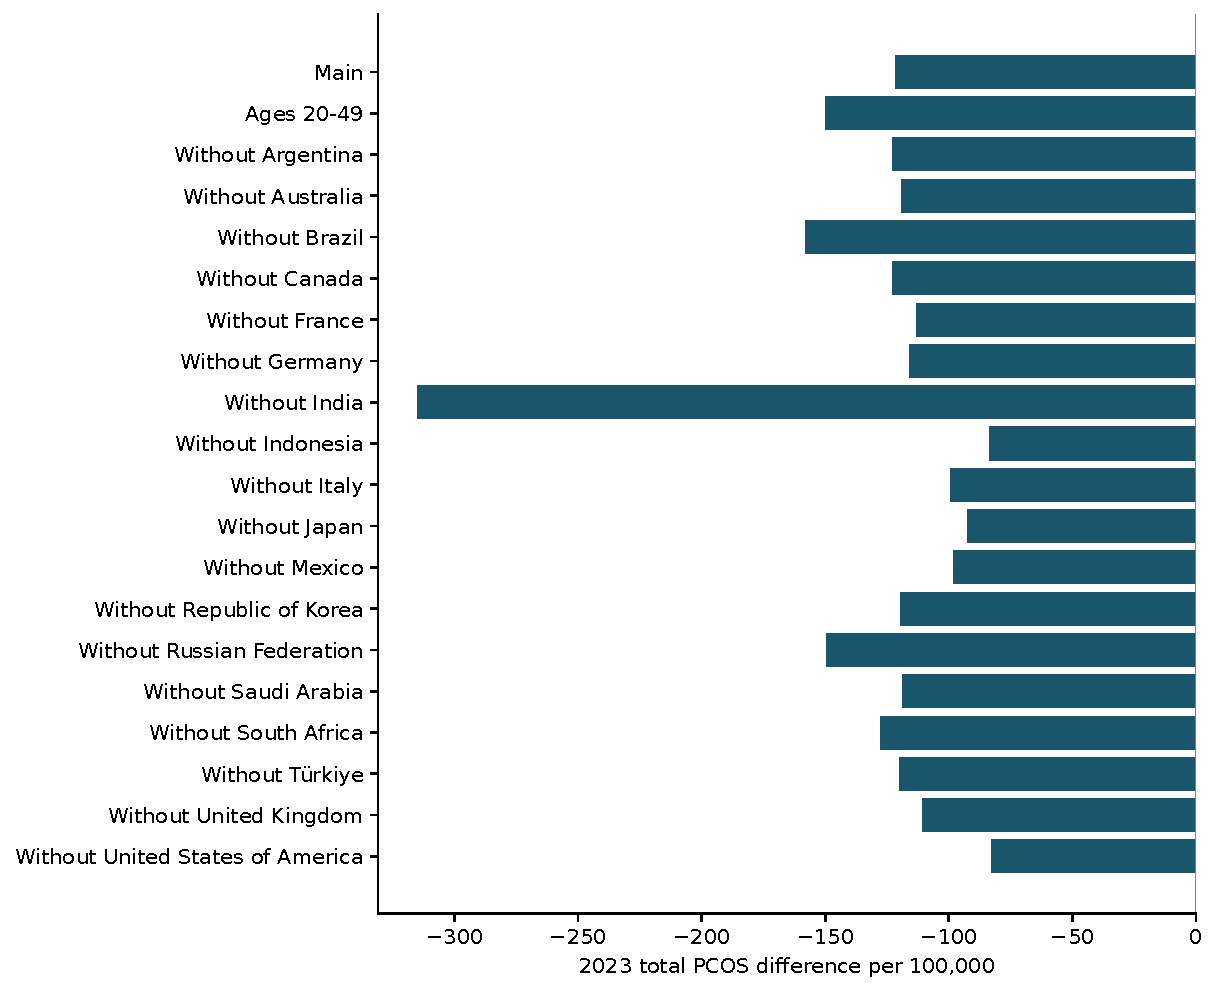
\includegraphics[width=.92\textwidth,height=.73\textheight,keepaspectratio]{figures/FigureS1_reference_exclusions.pdf}
\caption{\textbf{2023 total PCOS differences under country exclusions and age restriction.} GBD population shares; all values are point estimates.}\label{fig:s1}\end{figure}
\clearpage
\begin{figure}[p]\centering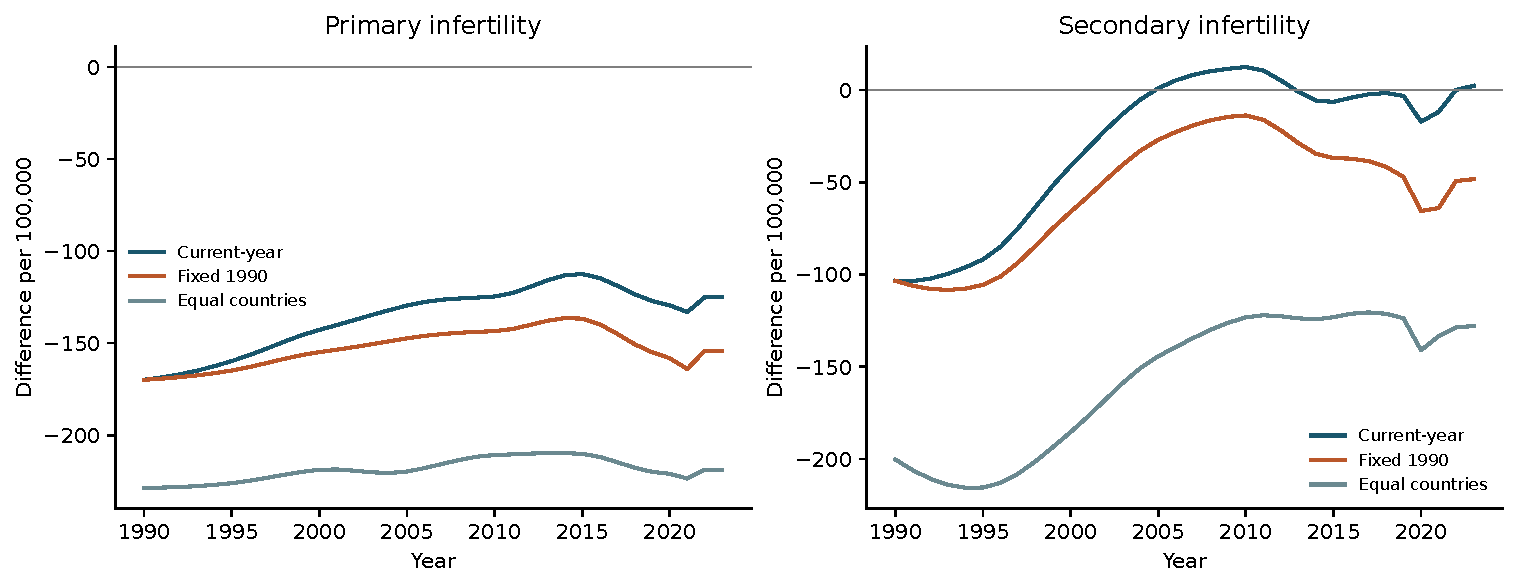
\includegraphics[width=.92\textwidth,height=.73\textheight,keepaspectratio]{figures/FigureS2_benchmark_trajectories.pdf}
\caption{\textbf{PCOS subtype differences under three benchmark definitions.} UN current-year shares, UN fixed-1990 shares and equal-country weights are applied within age. Disease rates remain GBD estimates.}\label{fig:s2}\end{figure}
\clearpage
\begin{figure}[p]\centering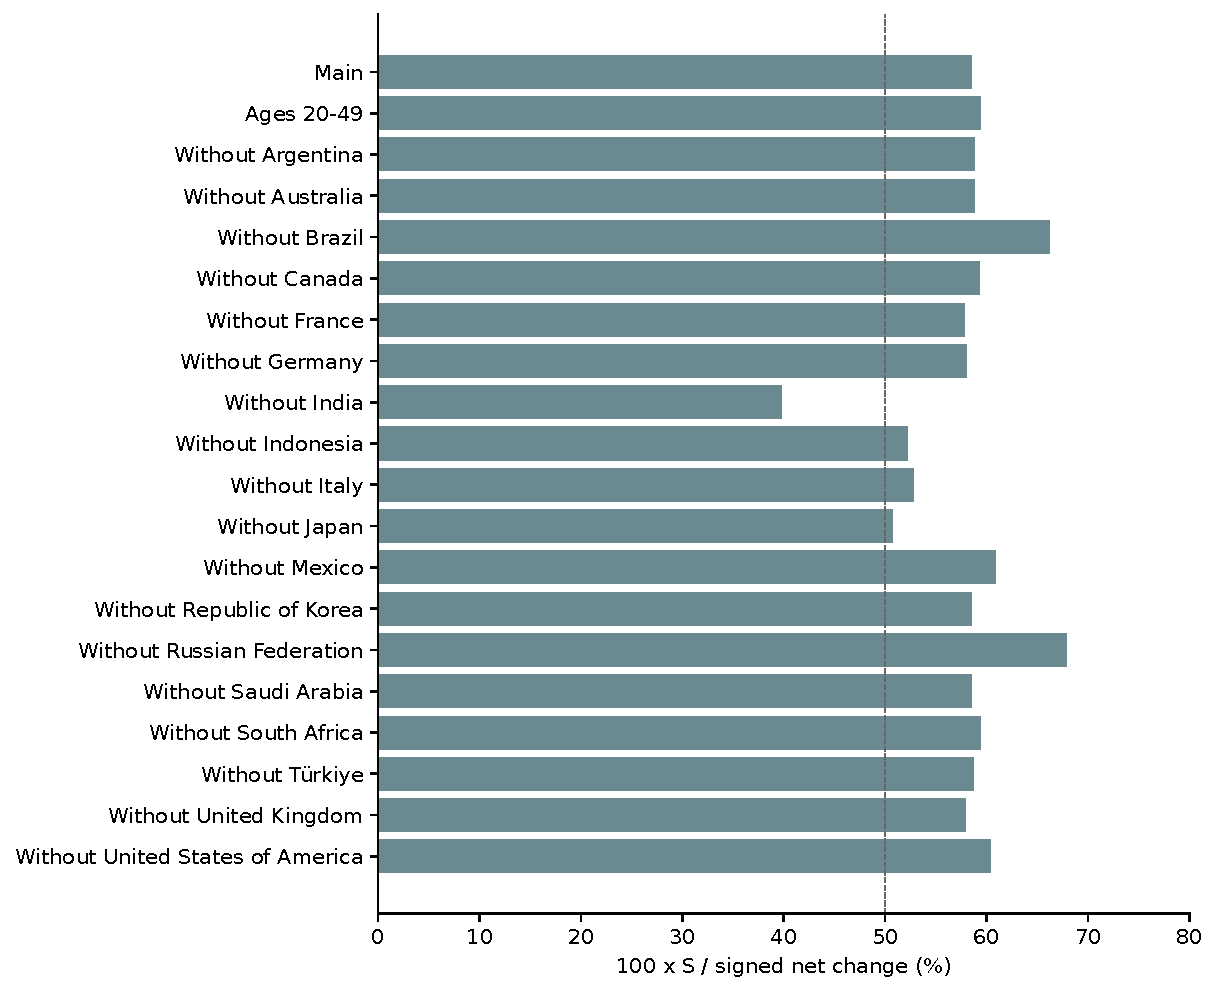
\includegraphics[width=.92\textwidth,height=.73\textheight,keepaspectratio]{figures/FigureS3_composition_sensitivity.pdf}
\caption{\textbf{Signed PCOS composition ratios under reference and age specifications.} The dashed line marks 50 percent, not a significance threshold. The 39.8--67.9 percent range is not a posterior interval.}\label{fig:s3}\end{figure}
\clearpage
\begin{figure}[p]\centering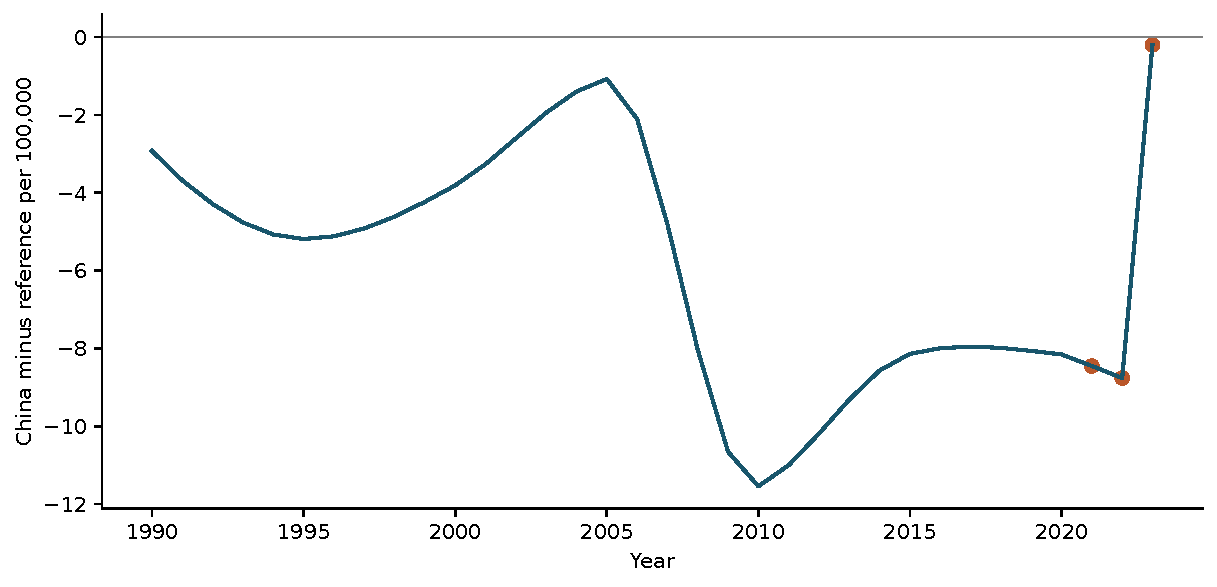
\includegraphics[width=.92\textwidth,height=.73\textheight,keepaspectratio]{figures/FigureS4_endometriosis_trajectory.pdf}
\caption{\textbf{Endometriosis total-infertility China-minus-reference trajectory.} The highlighted endpoints show why the 2023 near-zero contrast does not summarize a stable trajectory.}\label{fig:s4}\end{figure}
\clearpage
\begin{figure}[p]\centering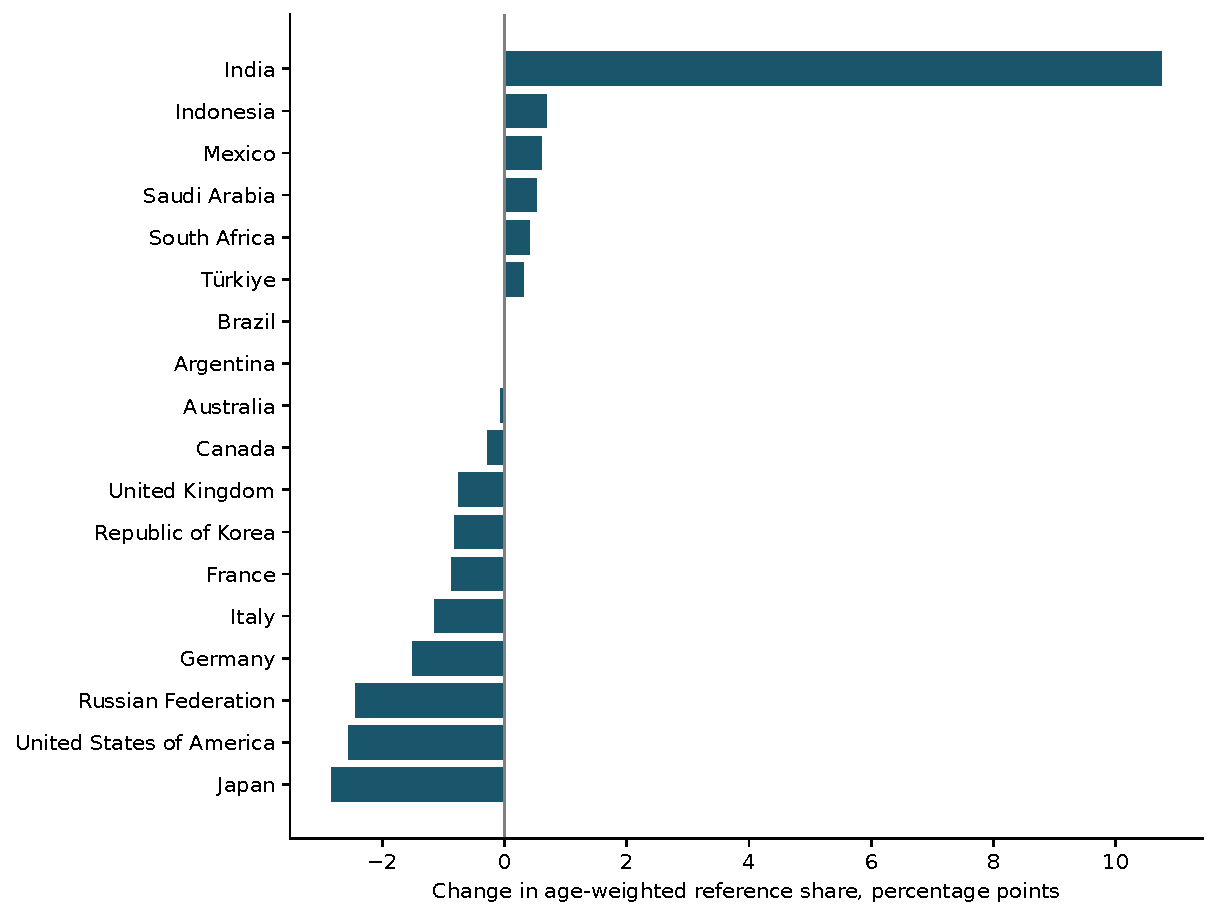
\includegraphics[width=.92\textwidth,height=.73\textheight,keepaspectratio]{figures/FigureS5_country_shifts.pdf}
\caption{\textbf{Changes in age-weighted reference-country shares, UN WPP 2024.} Country proportions within age are averaged with fixed standard age weights. These are composition changes, not disease-rate changes.}\label{fig:s5}\end{figure}
\clearpage
\begin{figure}[p]\centering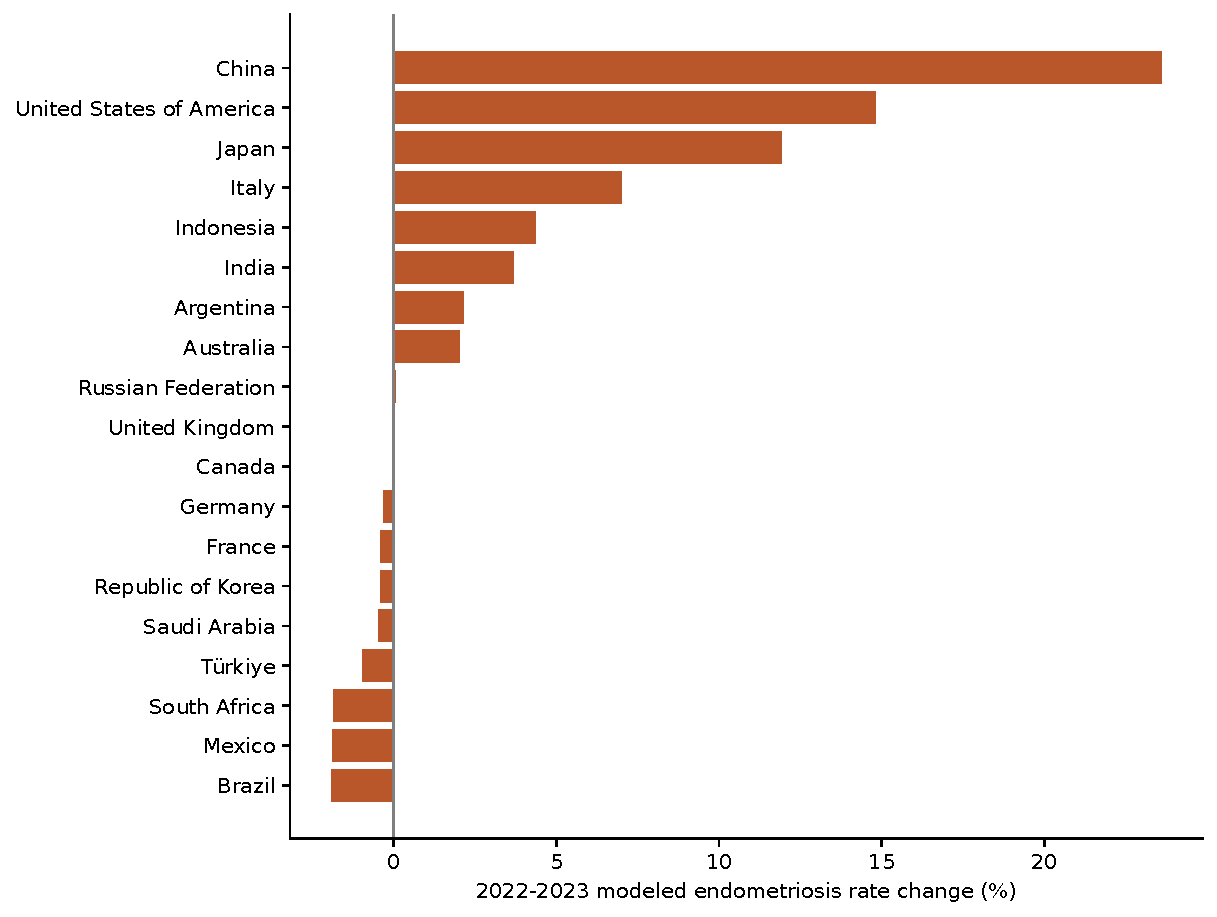
\includegraphics[width=.92\textwidth,height=.73\textheight,keepaspectratio]{figures/FigureS6_terminal_country.pdf}
\caption{\textbf{Endometriosis modeled rate changes across 19 countries, 2022--2023.} This reproduces the source release. It does not establish an epidemiological event or external validation.}\label{fig:s6}\end{figure}
\clearpage
\begin{figure}[p]\centering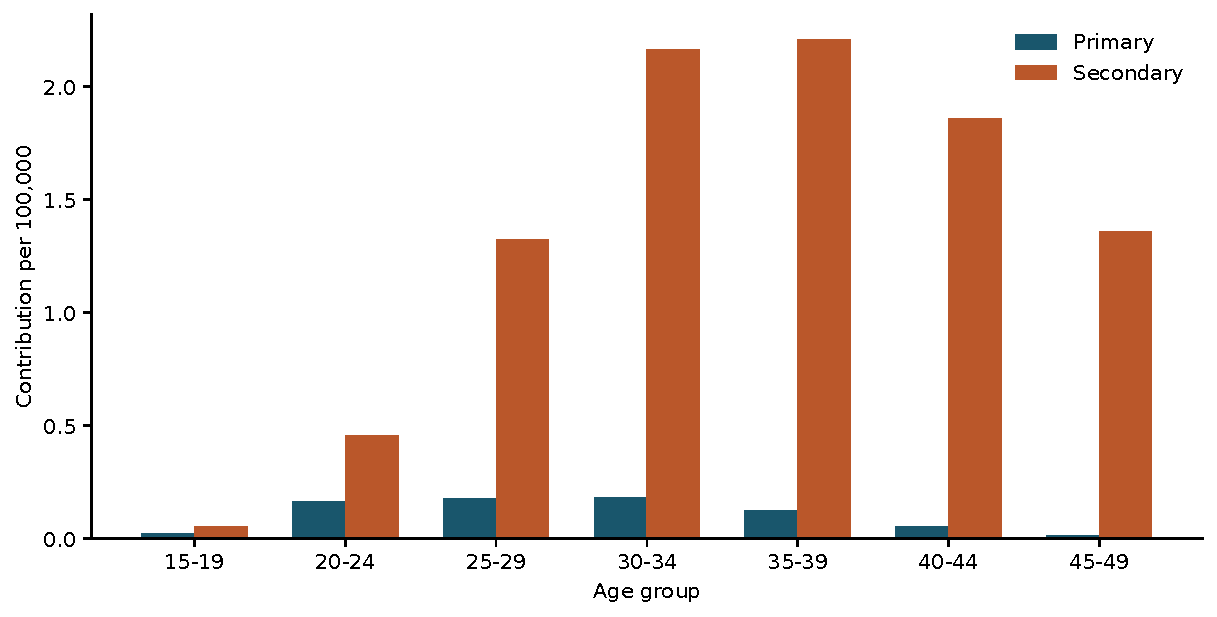
\includegraphics[width=.92\textwidth,height=.73\textheight,keepaspectratio]{figures/FigureS7_terminal_age_type.pdf}
\caption{\textbf{Age and infertility-type contributions to the Chinese endometriosis rate increment, 2022--2023.} Standard-weighted contributions sum to +10.1723 per 100,000. Most of the signed modeled increment is secondary infertility; this is not an etiologic fraction.}\label{fig:s7}\end{figure}
\clearpage
\end{document}
